%BAB_3 LAPORAN KP

\chapter{PERANCANGAN SISTEM}
Pada bab ini akan disajikan mekanisme perancangan alat baik perangkat keras ataupun perangkat lunak. Tahapan perancangan dimulai dari perancangan blok diagram sistem, perancangan perangkat keras, perancangan perangat lunak, perancangan kinematika, perancangan antarmuka, dan integrasi keseluruhan program. 
\section{ Blok Diagram Sistem }
Secara garis besar pada tahapan implementasi dari kinematika pada robot lengan SCARA Serpent ini menggunakan \textit{output} atau penggerak berupa motor DC dengan \textit{feedback} posisi berupa potensiometer sedangkan pada bagian  \textit{input} yang berasal dari GUI yang dibuat pada Processing IDE. Processing IDE nantinya mengirimkan sebuah koordinat yang digunakan untuk menentukan pergerakan robot berdasarkan fungsi \textit{invers kinematic}. Gambar \ref{pic.diagram.bloksistem} merupakan diagram blok sistem secara keseluruhan.
\begin{figure}[H]
	\centering
	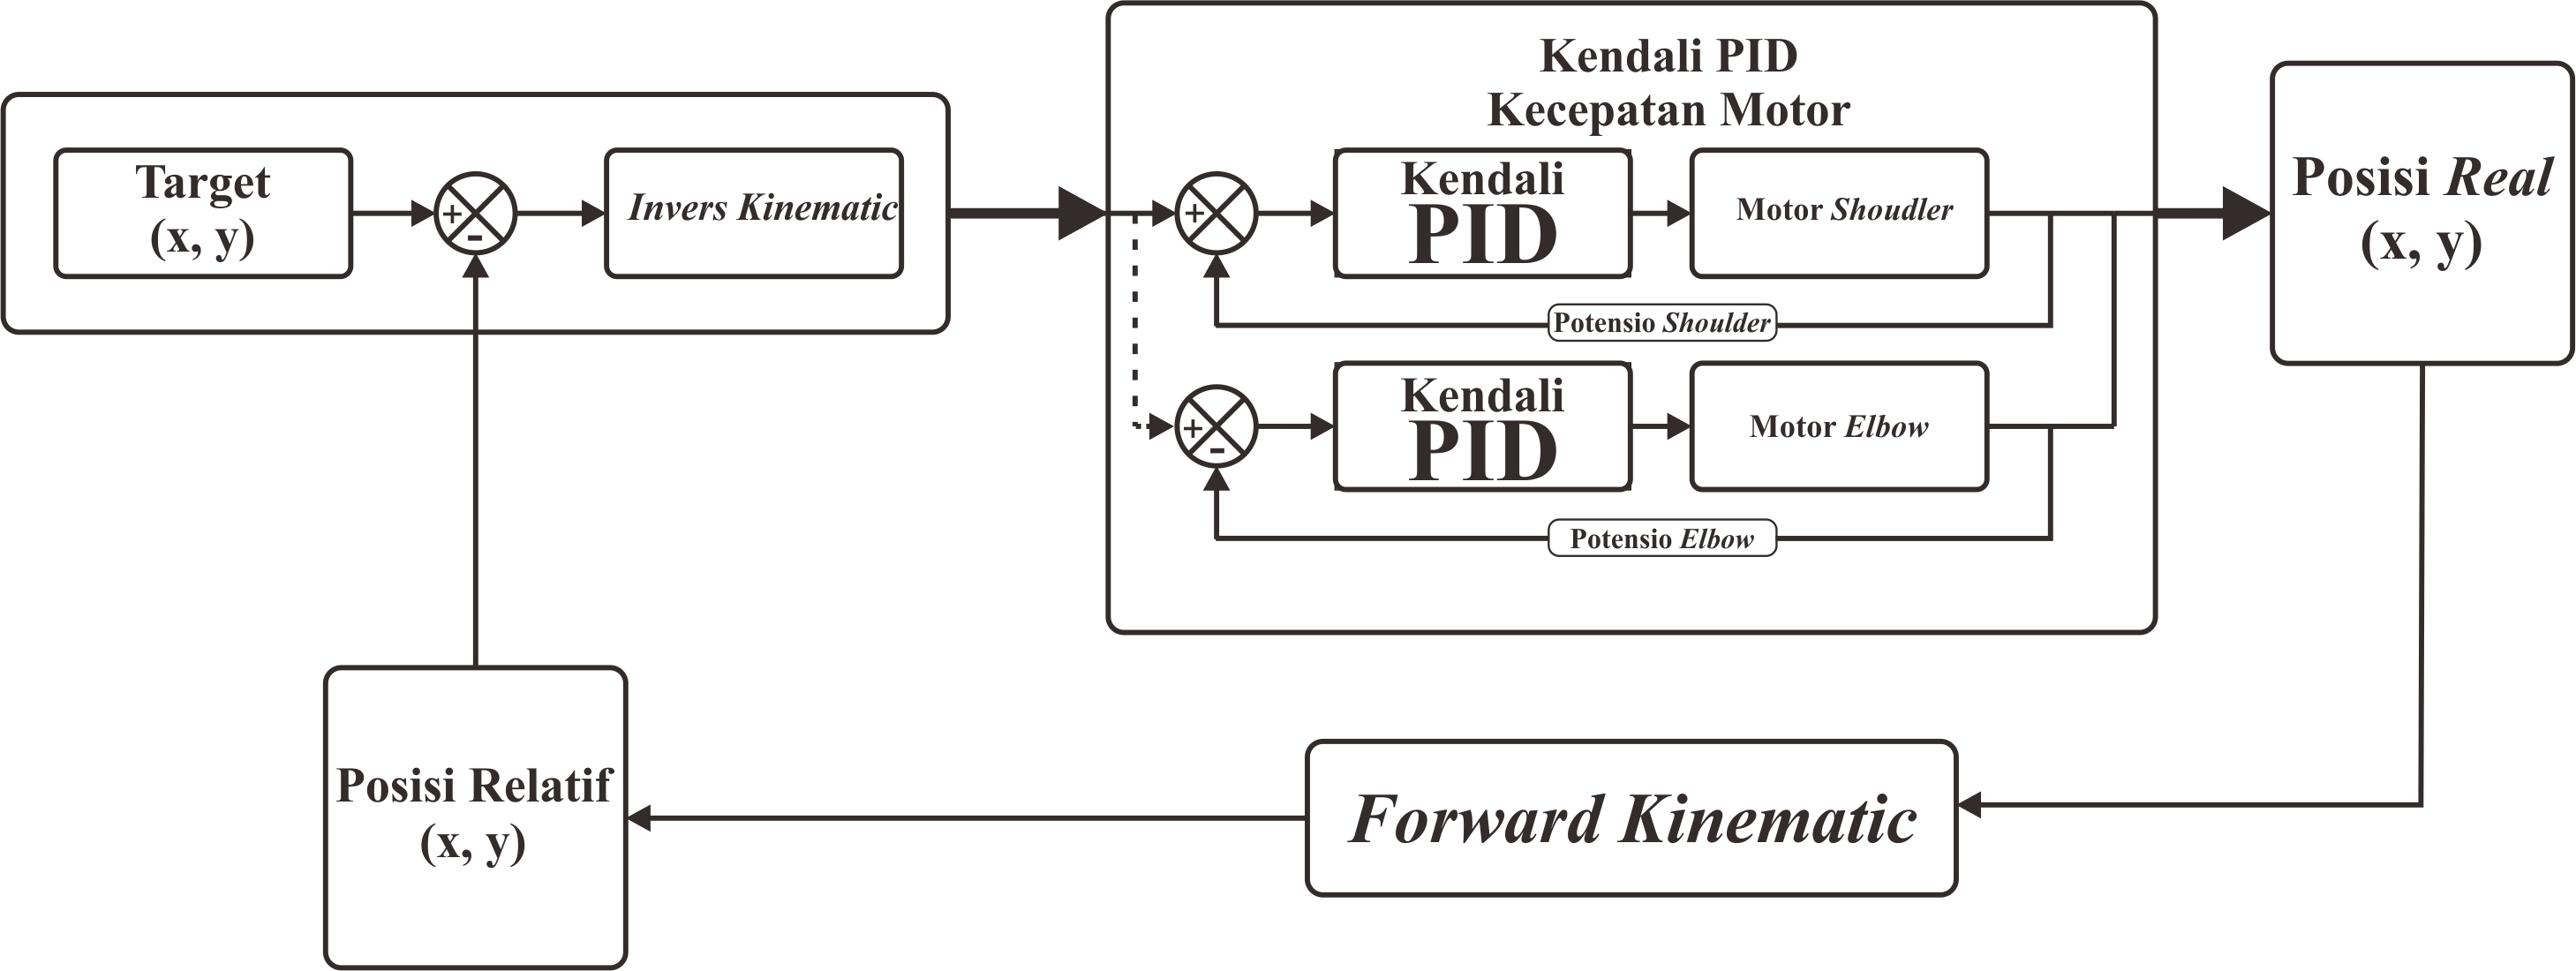
\includegraphics[width=13cm]{gambar/diagram_blok_new.png}
	\caption{Blok Diagram Sistem}
	\label{pic.diagram.bloksistem}
\end{figure}
Pada blok diagram yang disajikan pada Gambar \ref{pic.diagram.bloksistem} sistem terdiri dari bagian yang meliputi bagian masukan, bagian kendali, bagian keluaran, dan bagian penampil. Pada bagian masukan menggunakan GUI yang dirancang pada Processing IDE yang digunakan sebagai \textit{forward kinematic} serta \textit{inverse kinematic} dimana robot akan bergerak menyesuaikan dengan posisi atau sudut yang dimasukan melalui Processing IDE. 
Pada bagian kontrol menggunakan Arduino Mega 2560 sebagai mikrokontroler yang mengendalikan seluruh operasi dari robot. \textit{ Supply} Arduino sebesar 5 volt DC didapatkan dari regulator tegangan yang menurunkan tegangan dari 24 volt DC ke 5 volt DC. 

Pada bagian keluaran, pin \textit{pulse with modulation} (PWM) pada Arduino Mega 2560 dihubungkan dengan \textit{driver} motor yang digunakan untuk mengontrol arah pergerakan dari motor DC serta kecepatan pergerakan dari motor DC. Pergerakan arah putaran motor DC bergantung pada \textit{feedback} posisi setiap sendi yang diberikan oleh potensiometer. Tiga buah pin digital pada Ardunio Mega 2560 dihubungkan pada rangkaian \textit{switch} yang menggunakan IC TIP31 yang berfungsi sebagai kontrol dari \textit{end-effector} yang dioperasikan menggunakan tekanan udara yang dikontrol oleh \textit{valve pneumatic.}

Pada bagian penampil merupakan bentuk dari rancangan GUI yang dirancang dalam Processing IDE melalui sebuah bentuk pemrograman. Dalam tampilan GUI terdapat beberapa \textit{tools} yang dapat untuk mengatur pergerakan robot SCARA Serpent. Pada GUI menampilkan nilai dari sudut, dan posisi serta animasi robot SCARA Serpent pada kondisi langsung dari pergerakan robot SCARA Serpent.
\section{ Perancangan Perangkat Keras }
Perancangan perangkat keras pada robot lengan SCARA Serpent terdiri dari dua bagian yaitu bagian mekanis dan elektronis. Bagian  mekanis merupakan bagian \textit{hardware} yang meliputi desain, bahan dan bentuk dari\textit{ arm manipulator robot} SCARA Serpent. Bagian elektronis merupakan bagian \textit{hardware} yang meliputi sistem yang berkaitan dengan rangkaian elektronis pada robot SCARA Serpent seperti rangkaian pada desain \textit{board} serta komponen elektronis pendukung.
\subsection{ Sistem Mekanis }
Sistem memkanis dari robot lengan bergantung dari konfigurasi robot lengan. Konfigurasi robot lengan terbagi menjadi enam, yaitu konfigurasi \textit{articulated}, konfigurasi SCARA Serpent, konfigurasi \textit{spherical}, konfigurasi \textit{cylindrical}, dan konfigurasi \textit{cartesian}. Pada peneltian kerja praktik, konfigurasi robot lengan yang digunakan adalah konfigurasi SCARA Serpent dengan dua \textit{joint} \textit{revolute} dan satu \textit{joint prismatic}. Sistem mekanik dari lengan robot tiga DOF sangat berpengaruh dan mendominasi sistem karena bentuk dan pergerakan dari mekanik akan mempengaruhi elektronis serta program. Sistem mekanik yang baik sangat mendukung dari pergerakan robot, oleh karena itu perancangan mekanik harus proporsional dari panjang setiap lengan, lebar serta tinggi robot. \textit{Free body} dari robot SCARA Serpent ditunjukkan pada Gambar \ref{pic.freebodySCARA}. Bentuk fisik dari robot SCARA Serpent yang digunakan pada penelitian ini ditunjukkan pada Gambar \ref{pic.fisikSCARA}. 
\begin{figure}[H]
	\centering
	\includegraphics[width=7cm]{gambar/SCARAA.png}
	\caption{\textit{Free Body} Robot SCARA Serpent}
	\label{pic.freebodySCARA}
\end{figure}
\begin{figure}[H]
	\centering
	\includegraphics[width=9cm]{gambar/3dSCARA.png}
	\caption{Bentuk Fisik Robot SCARA Serpent}
	\label{pic.fisikSCARA}
\end{figure}
Robot SCARA Serpent merupakan robot yang meiliki tiga buah derajat kebebasan (DOF) yang terletak pada \textit{shoulder}, \textit{elbow}, dan \textit{end-effector}. Seluruh derajat kebebasan menggunakan sebuah motor DC yang didalamnya terdapat\textit{ gear box}. Motor DC pada \textit{end-effector} dibantu oleh sebuah \textit{belt} untuk menyalurkan putaran dari motor yang terletak pada atas \textit{shoulder}. Pergerakan pada masing-masing \textit{joint} memiliki jangkauan maksimum yang berbeda-beda. Jangkauan dipengaruhi oleh panjangnya lengan yang dimiliki oleh robot SCARA Serpent tersebut\cite{bulet}. Spesifikasi dari robot SCARA Serpent yang digunakan paad penelitian ini ditunjukkan pada Tabel \ref{tbl.elektronisSCARA}. 

\begin{longtable}{|c|l|}
	\caption{Sistem Elektronis SCARA Serpent}
	\label{tbl.elektronisSCARA}\\
	\hline
	\rowcolor[HTML]{9B9B9B} 
	Keterangan & \multicolumn{1}{c|}{\cellcolor[HTML]{9B9B9B}Nilai} \\ \hline
	\endfirsthead
	%
	\endhead
	%
	Panjang \textit{shoulder} & 360 mm                                             \\ \hline
	Panjgan \textit{elbow}  & 290 mm                                                    \\ \hline
	Gerakan \textit{shoulder}  &180 °                                  \\ \hline
	Gerakan \textit{elbow}  & 200 °                                  \\ \hline
	Rotasi \textit{end-effector}  & 360 °                                   \\ \hline
	Pergerakan naik dan turun \textit{end-effector}  &  150 mm                            \\ \hline
	Berat objek maksimum  &  3.0 kg                                                 \\ \hline
	
\end{longtable}

Desain pada\textit{ arm manipulator robot} SCARA Serpent berbahan besi dengan tebal 2 mm dengan tiga derajat kebebasan yang meliputi bagian \textit{shoulder}, \textit{elbow} serta \textit{end-effector}. Desain robot SCARA Serpent terbagi menjadi dua bagian. Bagian utama adalah \textit{box} panel yang berisi sistem elektronis utama dan pada bagian yang lain merupakan lengan dari robot SCARA Serpent sendiri. Terdapat juga tiga buah saluran udara yang berfungsi untuk mentransformasikan tekanan udara untuk pergerakan vertikal dari \textit{end-effector} yang berasal dari sebuah kompresor. Gambar \ref{pic.boxpanel} merupakan bentuk fisik dari box panel pada Robot SCARA Serpent.
\begin{figure}[H]
	\centering
	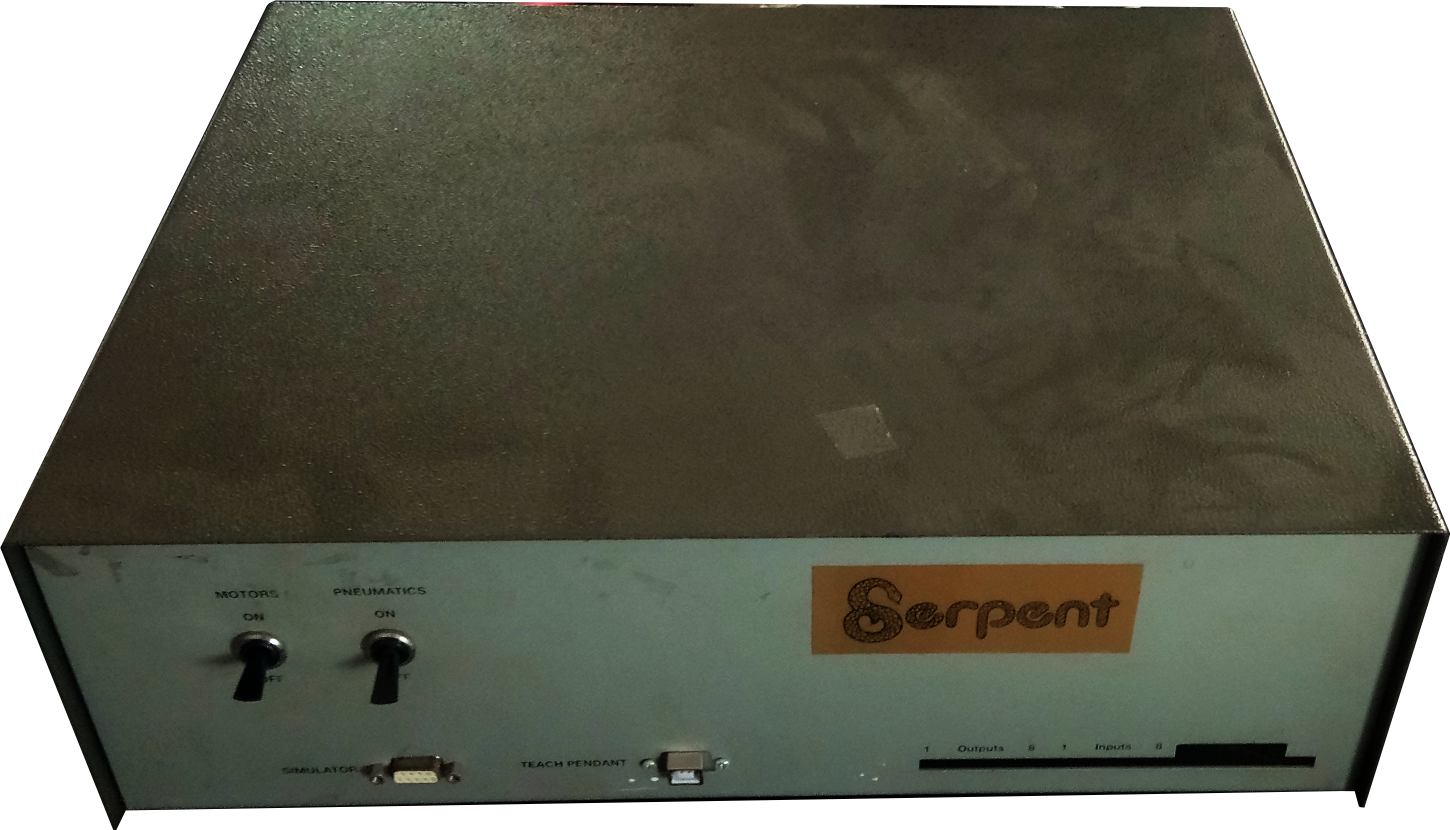
\includegraphics[width=9cm]{gambar/boxpanel.png}
	\caption{Box Panel Robot SCARA Serpent}
	\label{pic.boxpanel}
\end{figure}

Pada  SCARA Serpent menggunakan penggerak berupa motor DC 12 Volt dilengkapi dengan \textit{gearbox} sehingga mampu mengangkat beban berat karena torsi pada motor bertambah besar. Motor DC dikontrol oleh \textit{driver} motor EMS 30A H-\textit{Bridge} melalui Arduino Mega 2560. Spesifikasi dari motor DC yang digunakan pada robot SCARA Serpent ditunjukkan pada Tabel \ref{tbl.spesifikasimotordc}.
\begin{table}[H]
	\centering
	\caption{Spesifikasi Motor DC pada Robot SCARA Serpent}
	\label{tbl.spesifikasimotordc}
	\resizebox{15cm}{!}{%
		\begin{tabular}{|l|l|}
			\hline
			\rowcolor[HTML]{9B9B9B} 
			\multicolumn{1}{c|}{\cellcolor[HTML]{9B9B9B}Keterangan}		& \multicolumn{1}{c|}{\cellcolor[HTML]{9B9B9B}Nilai}			\\ \hline
			Momen inersia \textit{shoulder} ($J_{1}$)    							& $0.0980kgm^{2}$ 				\\ \hline
			Momen inersia \textit{elbow} ($J_{2}$)    							& $0.0115 kgm^{2}$ 				\\ \hline
			Massa \textit{shoulder}	($m_{1}$)											& $1.90kg$   					\\ \hline
			Massa \textit{elbow}  ($m_{2}$)     										& $0.93kg$   					\\ \hline
			Momen inersia motor ($J_{m}$)      								& $3.3*10^{-6}kgm^{2}$ 			\\ \hline
			GGL untuk motor \textit{shoulder} dan motor \textit{elbow }($K_{e1}=K_{e2}$)  		& $0.047Nm/A$   				\\ \hline
			Resistansi jangkar motor \textit{shoulder} dan \textit{elbow} ($R_{a1}=R_{a2}$)		& $3.5\Omega$  					\\ \hline
			Induktasnis jangkar motor \textit{shoulder} dan \textit{elbow}  ($L_{a1}=L_{a2}$) 		& $1.3mH$ 						\\ \hline
		\end{tabular}%
	}
\end{table}
%%
Pada bagian \textit{gearbox} pada masing-masing motor DC terdapat potensiometer yang pergerakan dari motor DC akan secara otomatis ikut bergerak dan kemudian mengirimkan nilai data analog ke Arduino Mega 2560. Data yang berhasil diterima oleh Arduino Mega 2560 kemudian diolah dan mendapatkan hasil berupa besar sudut pada pergerakan \textit{joint} tersebut. Bentuk fisik dari motor DC serta pemasangan potensiometer ditunjukkan pada Gambar \ref{pic.potensiometer}.
\begin{figure}[H]
	\centering
	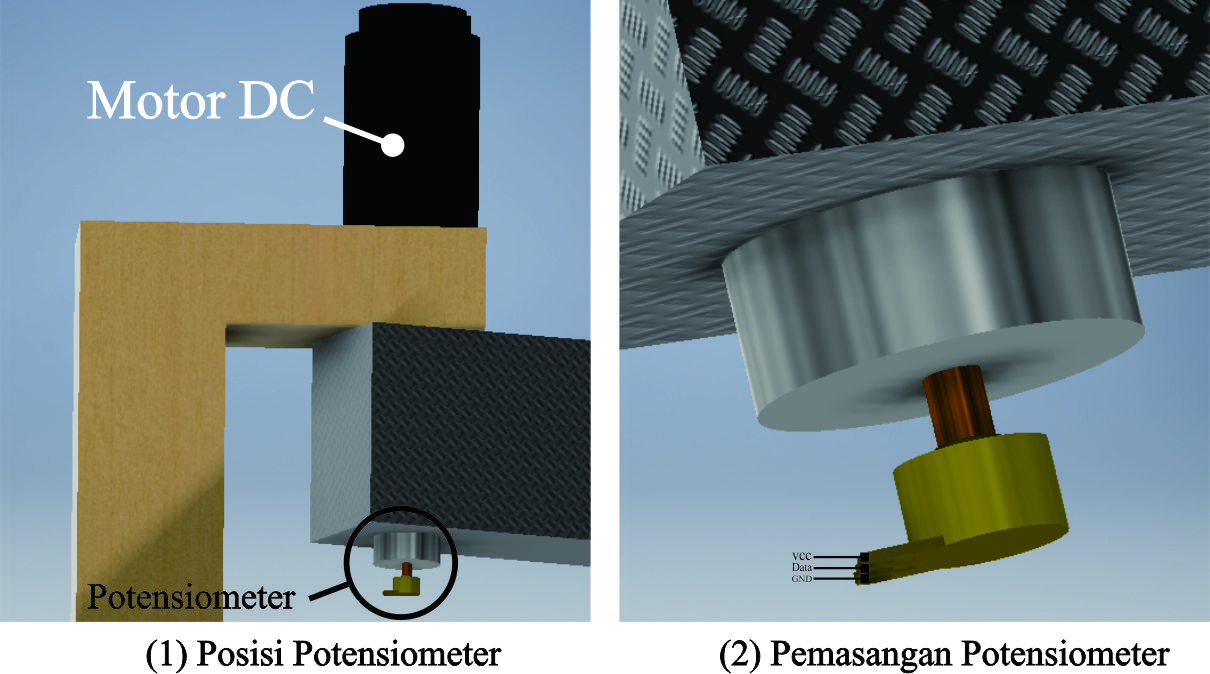
\includegraphics[width=10cm]{gambar/potsementara.jpg}
	\caption{Motor DC dengan potensiometer}
	\label{pic.potensiometer}
\end{figure}

Pada bagian \textit{end-effetor} menggunakan pergerakan translasi. Dengan pergerakan ini posisi \textit{end-effector} mengalami perubahan pada posisi tingginya. Pergerakan translasi juga terdapat pada bagian \textit{end-effector} yang menyebabkan sebuah \textit{gripper }\textit{ end-effector} dapat membuka dan menutup karena sebuah sistem mekanik yang telah ada di dalamnya. Selain dari pergerakan translasi, pergerakan pada \textit{end-effector} juga terdapat rotasi. Pergerakan ini dilakukan oleh satu buah motor DC yang ditempatkan pada bagian \textit{shoulder} dengan dihubungkan melalui sebuauh \textit{belt}. Pengoperasian pada motor DC ini juga dilakukan oleh \textit{driver} motor EMS 30A H-\textit{Bridge}. Bentuk fisik dari \textit{end-effector} pada robot SCARA Serpent ditunjukkan pada Gambar \ref{pic.endeffectorfisik}.
\begin{figure}[H]
	\centering
	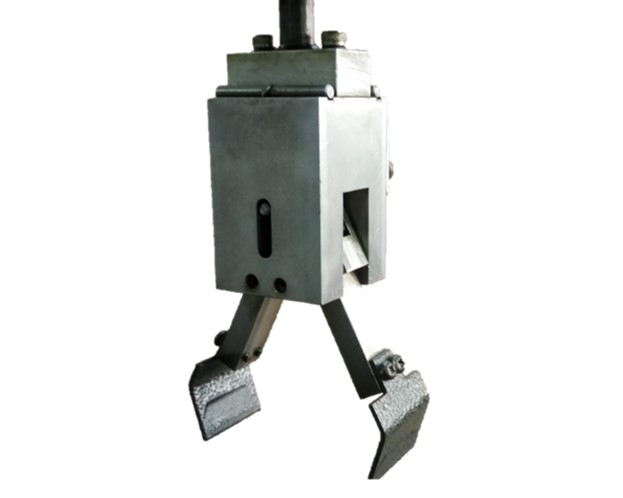
\includegraphics[width=6cm]{gambar/capitsementara.jpg}
	\caption{\textit{End-Effector} Robot SCARA Serpent}
	\label{pic.endeffectorfisik}
	
\end{figure}
Semua pergerakan pada \textit{end-effector} ditenagai oleh sebuah tekanan udara yang bersumber dari sebuah kompresor. Tekanan udara diaplikasikan pada sebuah \textit{pneumatic} dengan sistem kerja translasi yang dapat menyebabkan sebuah objek dapat bergerak pada sebuah garis lurus. Bentuk fisik dari \textit{pneumatic} robot SCARA Serpent ditunjukkan pada Gambar \ref{pic.pneumatic}.
\begin{figure}[H]
	\centering
	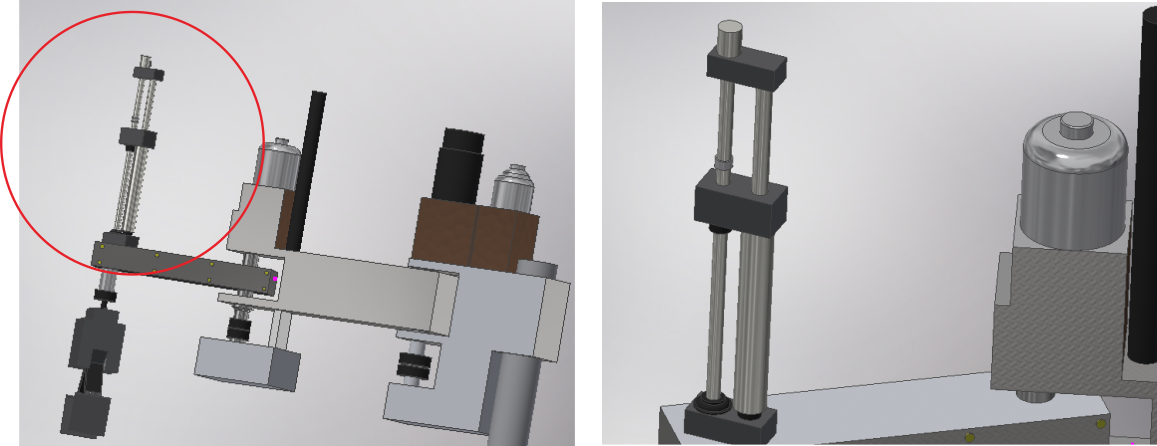
\includegraphics[width=11cm]{gambar/pneumatic.png}
	\caption{Bentuk Fisik \textit{Pneumatic}}
	\label{pic.pneumatic}
\end{figure}
Kompresor yang digunakan untuk menghasilkan sebuah tekanan udara merupakan sebuah kompresor listrik dengan kapasitas delapan bar. Kompresor ini dioperasikan menggunakan sumber tegangan AC 220 Volt. Bentuk fisik dari kompresor yang digunakan ditunjukkan pada Gambar \ref{pic.kompresor}.
\begin{figure}[H]
	\centering
	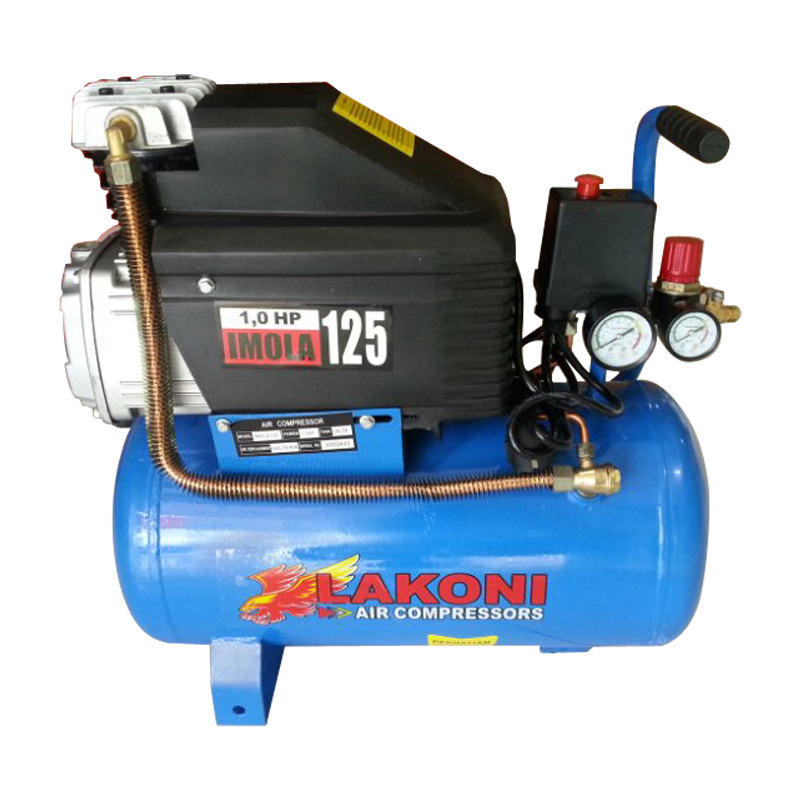
\includegraphics[height=5cm]{gambar/kompresor.png}
	\caption{Bentuk Fisik Kompresor}
	\label{pic.kompresor}
\end{figure}

Rancangan robot secara keseluruhan ditampilan pada Gambar \ref{pic.SCARAsamping} yang merupakan rancangan tampak samping dan Gambar \ref{pic.SCARAdimensi} merupakan rancangan dimensi robot. 
\begin{figure}[H]
	\centering
	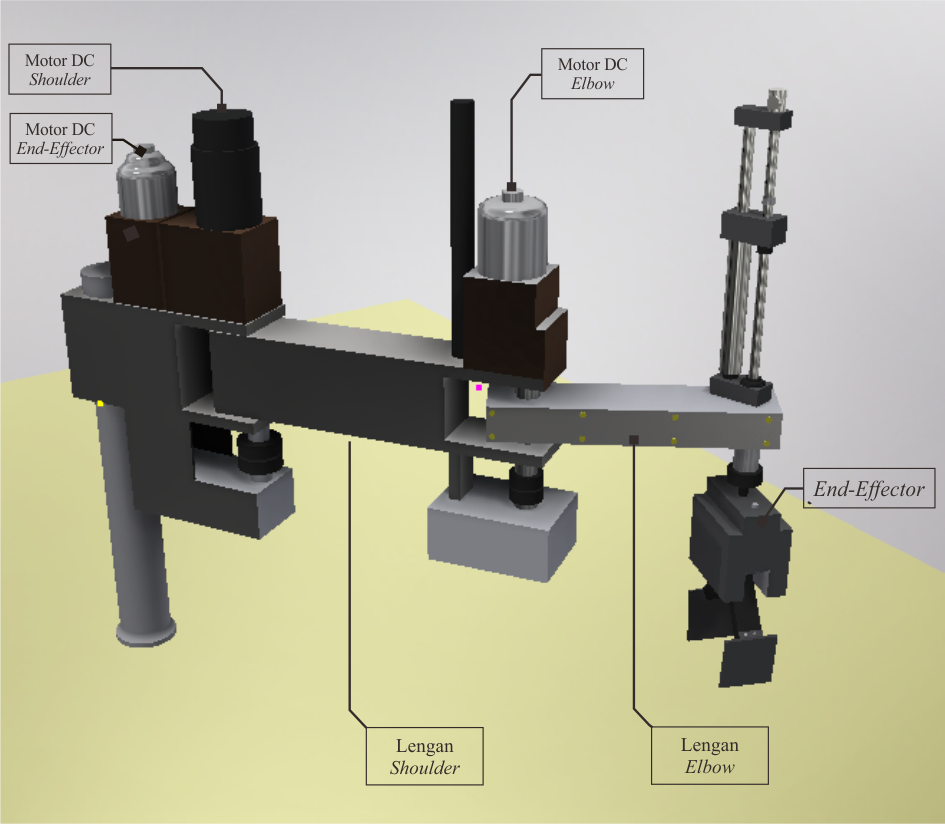
\includegraphics[height=9cm]{gambar/samping.png}
	\caption{Rancangan Tampak Samping}
	\label{pic.SCARAsamping}
\end{figure}

\begin{figure}[H]
	\centering
	\includegraphics[height=9 cm]{gambar/SCARAdimensi.png}
	\caption{Dimensi Robot}
	\label{pic.SCARAdimensi}
\end{figure}

\subsection{Rangkaian Elektronika}
\subsubsection{Rangkaian Motor DC}
Rancangan kendali pada robot lengan SCARA Serpent ini menggunakan tiga buah motor DC dengan masing – masing dilengkapi dengan \textit{gearbox} untuk memperkuat torsi yang dihasilkan oleh motor DC. Pada  \textit{gearbox} masing – masing motor  DC diberikan sensor potensiometer sebagai \textit{feedback} untuk memberikan posisi motor DC pada keseluruhan sistem. Motor DC diletakkan pada \textit{shoulder} untuk \textit{end-effector} satu buah yang dihubungkan melalui \textit{belt}, pada \textit{shoulder} satu buah, dan pada \textit{elbow} satu buah. Ketiga motor DC tersebut masing-masing menggunakan \textit{driver} motor EMS 30A H-\textit{Bridge} dalam sistem kerjanya. Pada masing – masing motor DC membutuhkan catu daya 12 Volt DC. Rangkaian \textit{driver} motor mendapat sumber tegangan DC 12V untuk disalurkan ke pada motor DC dan 5 Volt untuk kerja dari \textit{driver} motor sendiri. Tegangan keluaran sebesar 12 Volt yang dihasilkan oleh regulator \textit{buck} dengan sumber dari tegangan DC 24 Volt setelah dilakukan \textit{converter} AC to DC. Gambar \ref{pic.motordcdriver} merupakan Rangkaian Arduino Mega 2560 dengan \textit{Driver} Motor dan Motor DC.  

\begin{figure}[H]
	\centering
	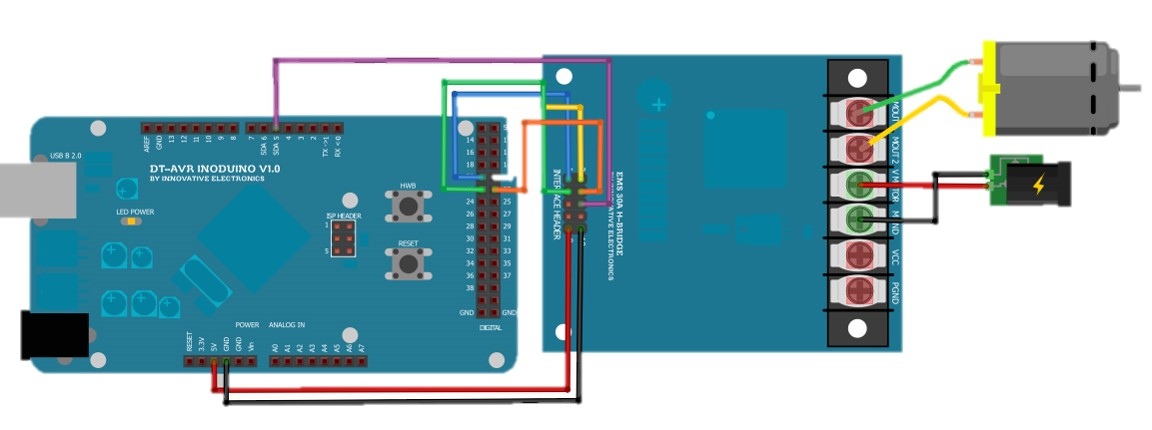
\includegraphics[width=10cm]{gambar/drivermotor.jpg}
	\caption{Rangkaian Arduino Mega 2560 dengan \textit{Driver} Motor dan Motor DC}
	\label{pic.motordcdriver}
\end{figure}
\subsubsection{Rangkaian \textit{Valve Pneumatic}}
\textit{End-effector} menggunakan tekanan udara dalam melakukan pergerakannya. Tekanan udara ini dikontrol menggunakan sebuah \textit{valve relay} dapat mengkontrol tekanan udara hingga delapan bar dan dapat bekerja pada tegangan DC 24 Volt. Tegangan 24 Volt pada \textit{valve relay} didapat dari keluaran dari rangkaian AC-DC yang dilakukan oleh dioda \textit{bridge} dengan masukan awalnya adalah tegangan AC 24 Volt yang diberikan oleh sebuah tranformator. Dengan besaran tegangan 24 Volt maka sebuah Arduino tidak dapat mengkontrolnya. Oleh karena itu, diberi sebuah rangkaian pembantu yang prinsipinya bekerja seperti saklar. Rangkaian tersebut dikontrol oleh IC TIP31 yang nantinya  menerima sinyal data digital dari Arduino Mega 2560 dan akan membuka jalur untuk tegangan 24 Volt. Gambar \ref{pic.fisikvalve} merupakan bentuk fisik dari \textit{valve relay} yang digunaakan dan Gambar \ref{pic.skematikvalve} merupakan rangkaian dari \textit{valve pneumatic} dengan rangkaian TIP31.
\begin{figure}[H]
	\centering
	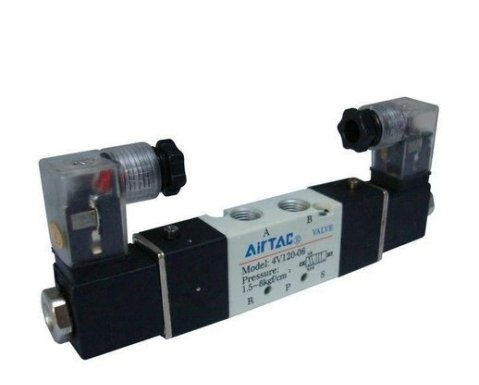
\includegraphics[width=5cm]{gambar/relay.jpg}
	\caption{Bentuk Fisik dari \textit{Valve Pneumatic}}
	\label{pic.fisikvalve}
\end{figure}
\begin{figure}[H]
	\centering
	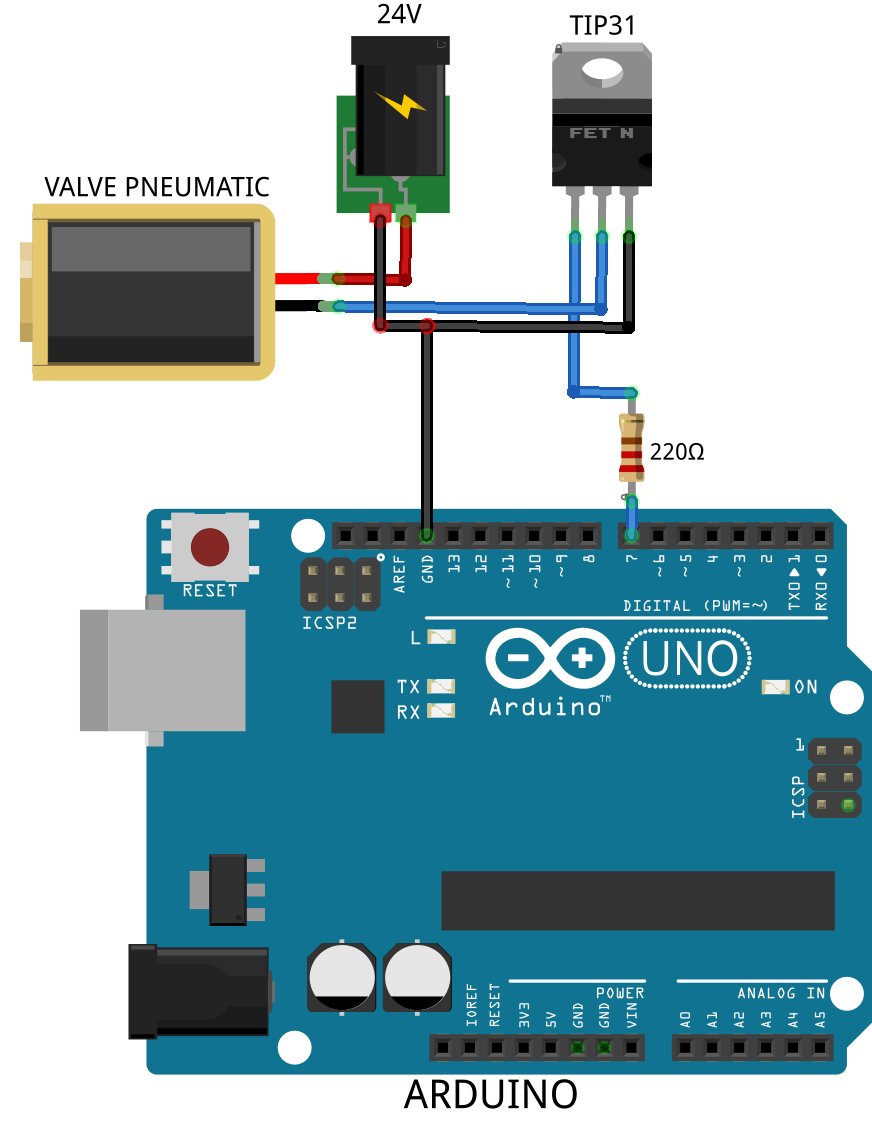
\includegraphics[width=5cm]{gambar/tip31.png}
	\caption{Rangkaian \textit{Valve Pneumatic} dengan Rangkaian TIP31}
	\label{pic.skematikvalve}
\end{figure}
\subsubsection{Sistem Elektronis Robot SCARA Serpent}
Arduino Mega 2560 digunakan sebagai mikrokontroler utama untuk mengendalikan seluruh sistem pada robot lengan SCARA Serpent. Arduino Mega 2560 memiliki banyak pin keluaran dan masukan digital dan analog yang dapat digunakan sebagai pengendali fungsi – fungsi dari setiap komponen. Pin pada Arduino  2560 dapat mencukupi kebutuhan masukan dan keluaran untuk sistem kerja robot. Pin \textit{analog} yang pada Arduino Mega 2560 digunakan untuk menerima \textit{feedback} masukkan dari potensiometer yang ada pada setiap motor. Beberapa pin digital pada Arduino Mega 2560 juga  memiliki fungsi lain yaitu sebagai pin \textit{pulse with modulation} (PWM) yang dapat digunakan sebagai keluaran analog sehingga dapat digunakan untuk mengatur nilai tegangan kaluaran dari Arduino  2560. Pin PWM yang cukup digunakan untuk kontrol kecepatan pada \textit{driver} motor. Selain itu pin PWM pada Arduino Mega 2560 digunakan untuk memberikan kontrol direksi pada \textit{driver} motor untuk memberikan masukan arah putar kanan ataupun putar kiri. Gambar \ref{pic.boxpanelkabel} merupakan sistem elektronis keseluruhan robot SCARA Serpent yang terdapat di dalam \textit{box} panel dan Tabel \ref{tbl.elektronisSCARA Serpent} merupakan keterangan dari masing-masing komponen.
\begin{figure}[H]
	\centering
	\includegraphics[width=13cm]{gambar/panelkabel.png}
	\caption{Sistem Elektronis Robot SCARA Serpent}
	\label{pic.boxpanelkabel}
\end{figure}
% Please add the following required packages to your document preamble:
% \usepackage[table,xcdraw]{xcolor}
% If you use beamer only pass "xcolor=table" option, i.e. \documentclass[xcolor=table]{beamer}
% \usepackage{longtable}
% Note: It may be necessary to compile the document several times to get a multi-page table to line up properly
\begin{longtable}{|c|l|}
	\caption{Sistem Elektronis SCARA Serpent}
	\label{tbl.elektronisSCARA Serpent}\\
	\hline
	\rowcolor[HTML]{9B9B9B} 
	No & \multicolumn{1}{c|}{\cellcolor[HTML]{9B9B9B}Keterangan} \\ \hline
	\endfirsthead
	%
	\endhead
	%
	1  & \textit{Conncetor} utama                                          \\ \hline
	2  & Kipas                                                     \\ \hline
	3  &\textit{Valve relay pneumatic}                                   \\ \hline
	4  &\textit{Switch} motor dan \textit{pneumatic}                              \\ \hline
	5  & \textit{Connector remote  }                                      \\ \hline
	6  & \textit{Connector} Arduino Mega 2560                             \\ \hline
	7  & \textit{Board} utama                                             \\ \hline
	8  & \textit{Driver} motor EMS 30A H-\textit{Brdige}                           \\ \hline
	9  & Transformator                                           \\ \hline
	10 & \textit{Swtich} AC                                               \\ \hline
	11 & \textit{Connector} AC                                            \\ \hline
\end{longtable}

Pada Gambar \ref{pic.boxpanelkabel} terlihat bahwa sistem elektronis dari robot SCARA Serpent mempunyai kontrol utama yang terdiri dari Arduino Mega 2560 dan terdapat beberapa komponen pendukung. Gambar \ref{pic.sisminarduino} merupakan rangkaian elektronis utama dari robot SCARA Serpent yang disajikan melalui 3D Fusion dan Tabel \ref{tbl.pinarduino} merupakan fungsi dari masing-masing pin Arduino Mega 2560.
\begin{figure}[H]
	\centering
	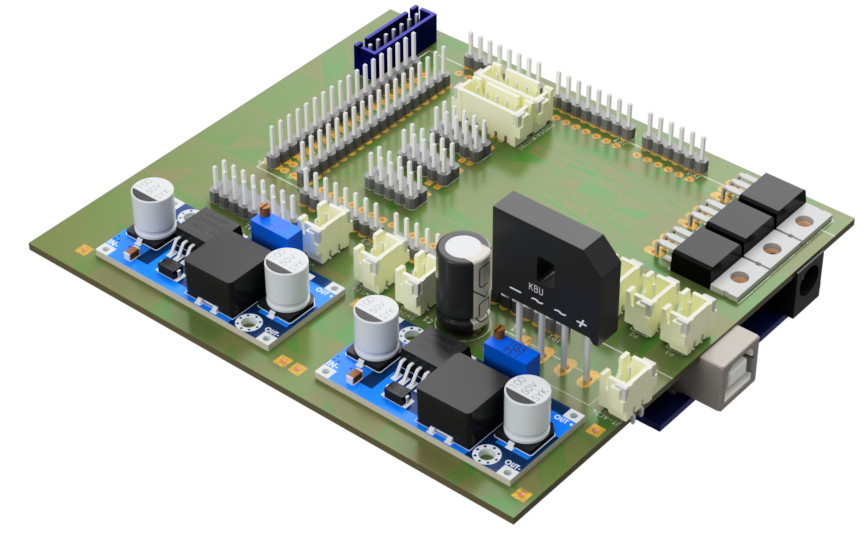
\includegraphics[width=10cm, height=10cm]{gambar/fusion.png}
	\caption{3D Fusion Rangkaian Elektronis}
	\label{pic.sisminarduino}
\end{figure}

% Please add the following required packages to your document preamble:
% \usepackage[table,xcdraw]{xcolor}
% If you use beamer only pass "xcolor=table" option, i.e. \documentclass[xcolor=table]{beamer}
% \usepackage{longtable}
% Note: It may be necessary to compile the document several times to get a multi-page table to line up properly
\begin{longtable}{|c|c|l|}
	\caption{Fungsi Arduino Mega 2560}
	\label{tbl.pinarduino}\\
	\hline
	\rowcolor[HTML]{656565} 
	{\color[HTML]{000000} No} & {\color[HTML]{000000} Pin Arduino Mega 2560} & \multicolumn{1}{c|}{\cellcolor[HTML]{656565}{\color[HTML]{000000} Fungsi}} \\ \hline
	\endfirsthead
	%
	\endhead
	%
	1                         & A1                                 & \textit{Feedback} potensiometer \textit{shoulder}                                            \\ \hline
	2                         & A2                                 & \textit{Feedback} potensiometer \textit{elbow}                                               \\ \hline
	3                         & A3                                 & {\color[HTML]{000000} \textit{Feedback} potensiometer \textit{end-effector}}                 \\ \hline
	4                         & D16, D18                           & Kontrol aktif \textit{driver} motor \textit{shoulder}                                        \\ \hline
	4                         & D20, D22                           & Kontrol \textit{driver} motor \textit{shoulder}                                              \\ \hline
	5                         & D24, D26                           & Kontrol aktif \textit{driver} motor \textit{elbow}                                           \\ \hline
	6                         & D28, D30                           & Kontrol \textit{driver} motor \textit{elbow}                                                 \\ \hline
	7                         & D32, D34                           & Kontrol aktif \textit{driver} motor \textit{end-effector  }                                  \\ \hline
	8                         & D36, D38                           & Kontrol \textit{driver} motor \textit{end-effector }                                         \\ \hline
	9                         & D4                                 & Kontrol PWM \textit{driver} motor \textit{shoulder}                                          \\ \hline
	10                        & D5                                 & Kontrol PWM \textit{driver} motor \textit{elbow}                                             \\ \hline
	11                        & D6                                 & Kontrol PWM \textit{driver} motor \textit{end-effector}                                      \\ \hline
	12                        & D7                                 & Kontrol \textit{valve relay} naik                                                   \\ \hline
	13                        & D8                                 & Kontrol \textit{valve relay} turun                                                  \\ \hline
	14                        & D9                                 & Kontrol \textit{valve relay} buka-tutup                                             \\ \hline
	15                        & D15                                & Kontrol LED \textit{Shoulder} aktif \textit{high}                                            \\ \hline
	16                        & D17                                & Kontrol LED \textit{elbow} aktif \textit{high}                                               \\ \hline
	17                        & D19                                & Kontrol LED \textit{end-effector} naik aktif \textit{high}                                   \\ \hline
	18                        & D21                                & Kontrol LED \textit{end-effector} turun aktif \textit{high}                                  \\ \hline
	19                        & D23                                & Kontrol LED \textit{end-effector} buka-tutup aktif \textit{high}                             \\ \hline
	20                        & D25                                & Buzzer aktif \textit{high}                                                          \\ \hline
\end{longtable}

\subsubsection{Rangkaian Catu Daya}
Rangkaian catu daya merupakan hal yang sangat penting dalam sebuah sistem. Pada robot lengan SCARA Serpent terdapat tiga buah nilai tegangan \textit{supply} yang berbeda. Tegangan yang ditujukkan untuk Arduino Mega 2560 dan beberapa sensor membutuhkan tegangan 5 Volt, motor DC membutuhkan tegangan 12 Volt dan \textit{valve pneumatic} membutuhkan tegangan 24 Volt. Catu daya diawali dengan tegangan AC 220 Volt dari listrik PLN. Tegangan tersebut kemudian diturunkan menggunakan sebuah trafo 5 Ampere menjadi 24 Volt AC. Komponen yang digunakan dalam rangkaian merupakan komponen yang membutuhkan tegangan DC, maka tegangan 24 Volt AC diubah menjadi 24 Volt DC menggunakan rangkaian dioda \textit{bridge}. Tegangan 24 Volt DC diarahkan menuju dua buah regulator \textit{buck} LM2596 yang masing-masing menghasilkan tegangan 12 Volt dan 5 Volt. Rangkaian catu daya secara keseluruhan ditunjukkan pada Gambar \ref{pic.skematikcatu}.
\begin{figure}[H]
	\centering
	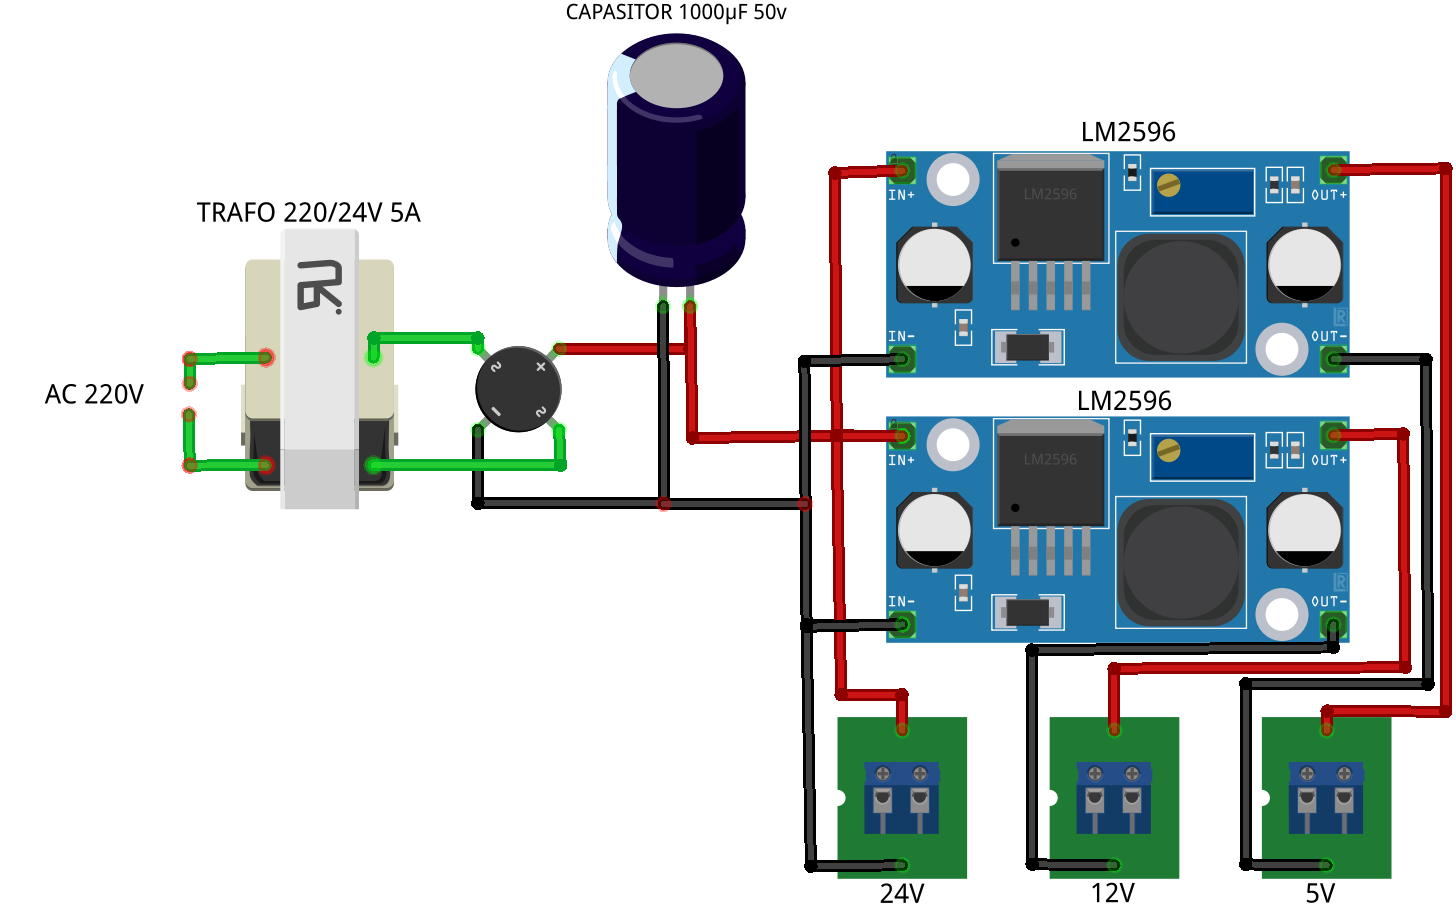
\includegraphics[width=8cm]{gambar/catudaya_bb.png}
	\caption{Rangkaian Catu Daya}
	\label{pic.skematikcatu}
\end{figure}
\section{Perancangan Perangkat Lunak}
Perangkat lunak yang digunakan merupakan \textit{software} Processing IDE. Processing IDE diprogram agar menghasilkan sebuah GUI yang cocok sesuai dengan fungsi robot SCARA Serpent. Di dalam GUI terdapat dua bagian yang diantaranaya merupakan bagian \textit{control} dan bagian \textit{display}. Pada bagian kontrol pada GUI berfungsi untuk mengkontrol mulai dari pergerakan dan posisi dari robot SCARA Serpent. Sedangkan pada bagian penampil, GUI menampilkan nilai dari sudut, posisi, serta animasi terkait robot SCARA Serpent. Gambar \ref{pic.gui} merupakan tampilan dari GUI secara keseluruhan. Setiap komponen yang ditampilan di dalam GUI processing IDE ditunjukkan pada Tabel \ref{tbl.gui}.
\begin{figure}[H]
	\centering
	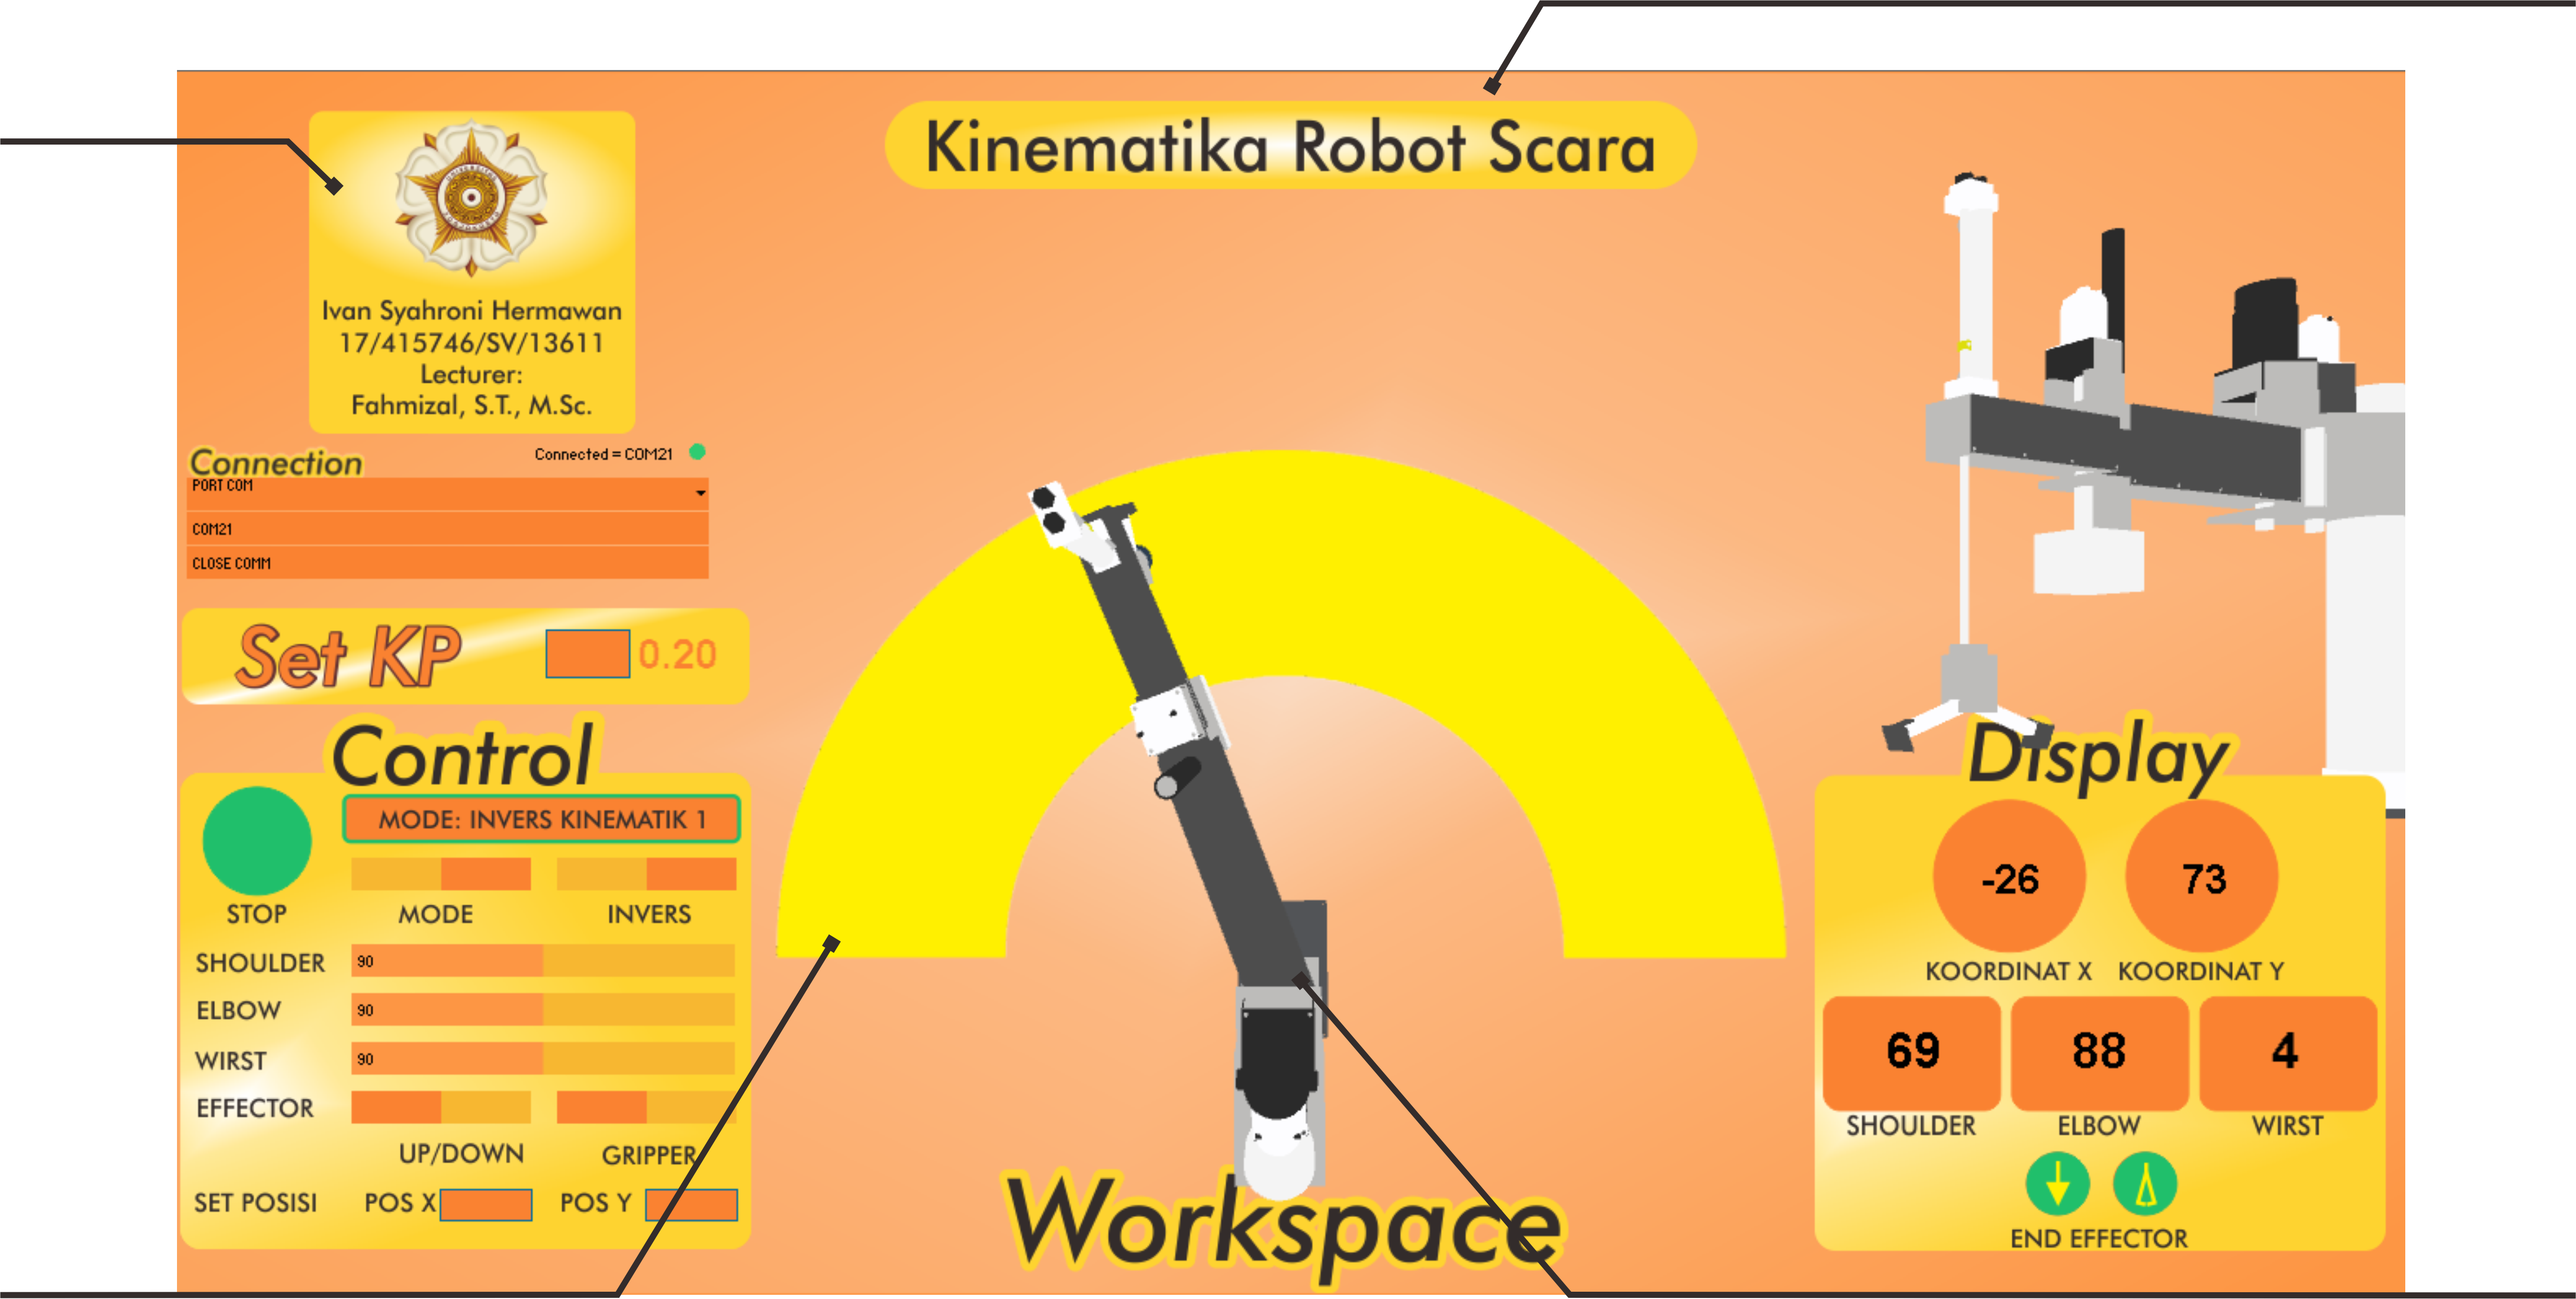
\includegraphics[width=12cm ]{gambar/GUI.png}
	\caption{Tampilan GUI Sistem Kinematika Robot SCARA Serpent}
	\label{pic.gui}
\end{figure}
% Please add the following required packages to your document preamble:
% \usepackage[table,xcdraw]{xcolor}
% If you use beamer only pass "xcolor=table" option, i.e. \documentclass[xcolor=table]{beamer}
% \usepackage[normalem]{ulem}
% \useunder{\uline}{\ul}{}
% \usepackage{longtable}
% Note: It may be necessary to compile the document several times to get a multi-page table to line up properly
\begin{longtable}{|c|l|l|}
	\caption{GUI Robot SCARA Serpent Serpent dengan Processing IDE}
	\label{tbl.gui}\\
	\hline
	\rowcolor[HTML]{9B9B9B} 
	No & \multicolumn{1}{c|}{\cellcolor[HTML]{9B9B9B}Nama} & \multicolumn{1}{c|}{\cellcolor[HTML]{9B9B9B}Fungsi}                                                             \\ \hline
	\endfirsthead
	%
	\endhead
	%
	1  & Identitas                                         & Menampilkan identitas                                                                                           \\ \hline
	2  & Koneksi                                           & \begin{tabular}[c]{@{}l@{}}Menentukan komunikasi dengan \textit{hardware} \\ yang akan dihubungkan\end{tabular} \\ \hline
	3  & Set kendali                                       & Memasukkan nilai kendai                                                                                         \\ \hline
	4  & Kelompok kontrol                                 & \begin{tabular}[c]{@{}l@{}}Terdiri dari beberapa kontrol untuk mengatur \\ pergerakan robot SCARA Serpent\end{tabular}  \\ \hline
	5  & Workspace                                         & Ruang kerja robot SCARA Serpent                                                                                         \\ \hline
	6  & \textit{3D Shape} tampak atas                              & \begin{tabular}[c]{@{}l@{}}Menampilkan pergerakan robot SCARA Serpent tampak \\ atas\end{tabular}                       \\ \hline
	7  & Tampilan data                                     & Menanmpilkan data-data terkait robot SCARA Serpent                                                                      \\ \hline
	8  & \textit{3D Shape} tampak samping                  & \begin{tabular}[c]{@{}l@{}}Menampilkan pergerakan robot SCARA Serpent tampak \\ samping\end{tabular}                    \\ \hline
	9  & Judul                                             & Judul dari antarmuka robot SCARA Serpent                                                                                \\ \hline
\end{longtable}
\subsection{ControlP5}
ControlP5 merupakan salah satu \textit{library} yang berguna dalam membuat sebuah GUI. Dalam \textit{library} yang disediakan terdapat banyak pilihan terkait kontrol sistem yang dapat digunakan. Kontrol sistem yang disediakan tersedia dua pilihan yaitu untuk menkontrol dan untuk menampilkan sebuah data. Masing-masing kontrol sistem ini dapat digunakan dengan cara memanggilnya pada program yang ditulis.

Pada perancangan kinematika robot SCARA Serpent, menggunakan empat buah kontrol sistem. Empat kontrol sistem yang digunakan merupakan jenis kontrol sistem yang berguna untuk memberikan sebuah data yang dikirimkan pada Arduino Mega 2560. Kontrol sistem tersebut diantaranya:
\begin{enumerate}
	\item \textit{Slider Control} \\
	\textit{Slider Control} berupa tampilan kontrol GUI yang menggunakan sistem geser dalam memberikan data. Data memiliki batasan atas dan batas bawah yang dimasukkan dalam program. Keuntungan menggunakan kontrol sistem jenis ini adalah mudahnya dalam memberikan sebuah data yang berbeda.
	
	
	\item \textit{Textfield Control} \\
	\textit{Textfield control} berupa tampila kontrol GUI yang menggunakan masukan nilai data sesuai apa yang dituliskan atau diketikkan secara langsung. Kelebihan menggunakan kontrol sistem jenis ini karena dapat memasukkan nilai data lebih spesifik secara langsung sesuai keiinginan.
	
	
	\item \textit{Toggle Control} \\
	\textit{Toggle control}
	\textit{Toggle control} memiliki sistem kontrol seperti saklar ON-OFF. Pada saat ditekan maka \textit{toggle control} menyimpan data berupa kondisi pertama dan berubah saat ditekan kembali. 
	
\end{enumerate}
\subsection{\textit{Shape}}
\textit{Shape} pada GUI berfungsi sebagai penampil animasi tiga dimensi dari robot SCARA Serpent. Robot SCARA Serpent dapat ditampilkan dalam berbagai ukuran, letak dan juga dapat bergerak sesuai dengan data yang diberikan. Pergerakan dari robot SCARA Serpent merupakan implementasi dari wujud aslinya dengan pergerakan yang sama. Dalam pengoperasianya, desain dari robot SCARA Serpent yang ditampilkan harus dimasukkan ke dalam folder yang sama dengan program Processing IDE. File yang dapat ditampilkan merupakan file dengan jenis obj. yang berarti file objek. Pada program robot SCARA Serpent file dari dimensi tiga dari robot SCARA Serpent memiliki tiga buah file dimana ketiganya adalah \textit{base, shoulder}, dan \textit{elbow}. 

\section{Sistem Kinematika}
Persamaan kinematika terbagi dua, yaitu kinematika maju dan kinematika balik. Kinematika maju digunakan untuk menentukan posisi dan orientasi \textit{end-effector} apabila variabel sudut \textit{joint}-nya telah diketahui. Kinematika balik digunakan untuk mencari \textit{joint} robot dalam menentukan posisi dan orientasi dari \textit{end-effector.}
\subsection{Prinsip Kerja Kinematika Maju}
	Metode Denavit-Hartenberg (DH) merupakan metode yang menggabungkan proses perhitungan rotasi dan translasi menjadi sebuah matriks yang menyertakan nilai-nilai sudut putar dan jarak sendi dari sebuah lengan robot. Dalam beberapa aplikasi, metode Denavit-Hartenberg umumnya digunakan dalam perhitungan \textit{forward kinematics}. Dalam penelitian ini dirancang aplikasi yang menggunakan metode Denavit-Hartenberg untuk menghitung sudut-sudut tiap sendi pada sebuah lengan robot. Matrik Denavit-Hartenberg yang berisi perhitungan rotasi dan translasi digunakan untuk mendapatkan nilai nilai sudut untuk menggerakkan tiap motor sendi. Empat aturan \textit{frame} Denavit-Hartenberg yaitu Sumbu $z$ harus menjadi sumbu rotasi atau translasi dari sebuah \textit{joint}. Sumbu $x$ harus tegak lurus dari sumbu $z$ \textit{frame} sebelumnya. Sumbu $x$ harus memotong atau menyilang dari sumbu $z$ \textit{frame} sebelumnya. Sumbu $y$ harus digambarkan sesuai dengan aturan tangan kanan setelah sumbu $x$   dan sumbu $z$ setiap \textit{frame} digambarkan. Gambar \ref{dhSCARA} merupakan struktur dari konfigurasi SCARA Serpent.
\begin{figure}[H]
	\centering
	\includegraphics[width=9cm ]{gambar/SCARAdh.png}
	\caption{Konfigurasi Robot SCARA Serpent}
	\label{dhSCARA}
\end{figure}
Pada setiap \textit{joint} dari robot SCARA Serpent memiliki nomor dari 1 sampai 4 dengan digambarkan sebuah vektor $x, y, z$ pada masing-masing \textit{jointnnya} yang berfungsi untuk memudahkan dalam pengisian pada parameter DH. Vektor $x, y, z$ digambarkan sesuai dengan arah pergerakan pada masing-masing \textit{joint} dimana $z$ merupakan koordinat dari pergerakan \textit{joint} tersebut. Selanjutnya dengan mengikuti kaidah tangan kanan maka arah dari $x$ dan $y$ dapat diketahui. 

Pada saat vektor telah digambarkan pada keseluruhan \textit{joint}, langkah selanjutnya adalah menentukan parameter DH yang diawali dengan menentukan $\alpha_{i}. \alpha_{i}$ merupakan besar sudut yang terbentuk dari koordinat $z_{i}$ dengan $z_{i-1}$.  Dimulai pada \textit{joint} 1, $\alpha_{1}$ adalah 0 karena koordinat $z_{0}$ dan $z_{1}$ mempunyai arah yang sama sehingga sudut yang dihasilkan antara $z_{0}$ dan $z_{1}$ adalah 0.  Pada \textit{joint} 2 nilai pada $\alpha_{2}$ adalah 180 atau  $\pi$ karena arah dari  $z_{1}$ dan  $z_{2}$ mengarah ke arah yang berlawanan yang berarti memiliki sudut 180. Pada \textit{joint} 3 dan 4 memiliki nilai 0 karena koordinat $z_{2}$ dan $z_{3}$ dalam arah yang sama yang berarti tidak ada perbedaan sudut.

Pada langkah selanjutnya adalah menentukan nilai dari $a_{i}$ dan $d_{i}$. $a_{i}$ merupakan nilai panjang dari jarak koordinat  $z_{i}$  dan  $z_{i-1}$ . Sedangkan $d_{i}$ merupakan nilai panjang dari jarak koordinat $x_{i}$ dan $x_{i-1}$. Pada \textit{joint} 1 nilai dari $a_{1}$ adalah LS karena jarak antara $z_{1}$ dengan $z_{0}$ dapat direpresentasikan dengan panjang LS atau panjang dari lengan \textit{shoulder} dan untuk $d_{1}$ mempunyai nilai 0 karena koordinat $x_{0}$ dan $x_{1}$ tidak memiliki perbedaan pada sumbu $y$. Untuk \textit{joint} 2, nilai dari $a_{2}$ adalah Le atau lengan \textit{elbow} dikarenakan posisi dari koordinat $z_{1}$  dan $z_{2}$  memiliki jarak yang dapat direpresentasikan menjadi Le dan untuk  $d_{2}$ memiliki nilai 0 dikarenakan tidak ada perbedaan pada sumbu $y$ pada  $x_{1}$ dan  $x_{2}$.  Untuk \textit{joint} 3 memiliki $a_{3}$ memiliki nilai 0 karena koordinat $z$ berada pada sumbu yang sama sehingga tidak ada jarak dan untuk nilai $d_{3}$  memiliki nilai D1 karena jarak antara $x_{2}$ dan $x_{3}$ dapat direpresentasikan dengan D1 yang merupakan sebuah variabel. Untuk \textit{joint} terakhir yaitu \textit{joint} 4 nilai $a_{4}$ adalah 0 karena koordinat $z_{3}$ dan $z_{4}$ searah dan berada pada satu sumbu dan nilai dari $d_{4}$ adalah D2.

Langkah terakhir adalah menentukan nilai $\theta_{i}$ pada masing-masing \textit{joint} yang memiliki jenis \textit{joint}  \textit{revolute}. Pada robot SCARA Serpent \textit{joint revolute} berada pada \textit{joint} 1, \textit{joint} 2, dan \textit{joint} 4.  $\theta_{i}$ merupakan sebuah variabel yang nilainya dapat menyesuaikan kondisi dari robot. Nilai  $\theta_{i}$ ditempatkan pada koordinat $z_{i}$ yang merupakan sumbu dari setiap \textit{joint}. 

Setelah paramaeter DH telah ditentukan semuanya kemudian nilai-nilai dari masing-masing parameter dituliskan ke dalam bentuk tabel yang bertujuan untuk memudahkan saat akan dimasukkan ke dalam sebuah persamaan. Tabel parameter DH terdiri dari baris yang berisi tentang joint yang dimiliki oleh robot dan kolom yang merupakan parameter DH seperti $a_{i},\alpha_{i}, d_{1}, dan \theta_{i}$. Tabel parameter DH dari robot SCARA Serpent ditunjukkan pada Tabel \ref{dh.SCARA Serpent}. 

\begin{table}[H]
	\centering
	\caption{DH Parameter Robot SCARA Serpent}
	\label{dh.SCARA Serpent}
	
	\begin{tabular}{|c|c|c|c|c|}
		\hline
		\rowcolor[HTML]{9B9B9B} 
		Link & $a_{1}$ & $\alpha_{1}$ & $d_{1}$ & $\theta_{1}$ \\ \hline
		1    & LS & 0      & 0     & $\theta_{1}$     \\ \hline
		2    & LE & $\pi$    & 0     & $\theta_{2}	$     \\ \hline
		3    & 0     & 0      & D1 & 0          \\ \hline
		4    & 0     & 0      & D2 & $\theta_{4}$ \\ \hline
	\end{tabular}
	
\end{table}

Dari parameter DH yang ditunjukkan pada Tabel \ref{dh.SCARA Serpent} dapat diimplementasikan ke dalam sebuah transformasi matriks. Terdapat empat buah transformasi matriks yang masing-masing menunjukan dari pergerakan \textit{joint} yang kemudian dimasukkan ke dalam persaaama parameter DH. Persamaan \ref{pers.dhSCARA Serpent} merupakan persamaan utama dari metode DH yang dari persamaan tersebut dapat dikelompokkan menjadi empat transformasi matriks.
\begin{equation}
A_{1} = R_{z1\theta1}T_{z1d1}T_{x1a1}R_{x1\alpha1}
\label{pers.dhSCARA Serpent}
\end{equation}

Dari persaman \ref{pers.dhSCARA Serpent} dapat dibagi menjadi empat kelompok yang membentuk transformasi matriks. Ke empat transforamasi matriks ini di dapat dari matriks yang dimiliki oleh parameter DH seperti yang ditunjukkan pada Persamaan \ref{dh.full}. Ke empat matriks tersebut kemudian digabungkan dan membentuk satu buat transformasi matriks secara keseluruhan. Matriks secara keseluruhan digunakan dalam melakukan perhitungan kinematika maju.

\begin{equation}
A_{i} = \begin{bmatrix}
\cos\theta_{i} &  -\cos\alpha_{i}\sin\theta_{i}&  \sin\alpha_{i}\sin\theta_{i}& a_{1}\cos\theta_{i}\\ 
\sin\theta_{i}&  \cos\alpha_{i}\cos\theta_{i}&  -\sin\alpha_{i}\cos\theta_{i}& a_{1}\sin\theta_{i}\\ 
0&\sin\alpha_{i}  &\cos\alpha_{i}  &d_{1} \\ 
0 & 0 & 0 &1 
\end{bmatrix}
\label{dh.full}
\end{equation}

Persamaan \ref{dh.SCARA Serpent1}, \ref{dh.SCARA Serpent2}, \ref{dh.SCARA Serpent3}, dan \ref{dh.SCARA Serpent4} merupakan transformasi matriks dari masing-masing \textit{joint} dengan nilai-nilai yang sudah dimasukkan sesuai dengan matriks pada Persamaan \ref{dh.full}. Pada ke empat matriks $C_{i}$ mempresentasikan $\cos\theta_{i}$ dan $S_{i}$ mempresentasikan $\sin\theta_{i}$.
\begin{equation}
A_{1} = \begin{bmatrix}
C_{1} &  -S_{1}&  0& a_{1}C_{1}\\ 
S_{1}&  C_{1}&  0& a_{1}C_{1}\\ 
0&0  &1  &0 \\ 
0 & 0 & 0 &1 
\end{bmatrix}
\label{dh.SCARA Serpent1}
\end{equation}

\begin{equation}
A_{2} = \begin{bmatrix}
C_{2} &  S_{2}&  0& a_{2}C_{2}\\ 
S_{2}&  -C_{2}&  0& a_{2}C_{2}\\ 
0&0  &-1  &0 \\ 
0 & 0 & 0 &1 
\end{bmatrix}
\label{dh.SCARA Serpent2}
\end{equation}


\begin{equation}A_{3}=\begin{bmatrix}
1 & 0 &0  &0 \\ 
0&1  &0  &0 \\ 
0 &0  &1  &d_{3} \\ 
0&0  &0  &1 
\end{bmatrix} 
\label{dh.SCARA Serpent3}
\end{equation}

\begin{equation}
A_{4} = \begin{bmatrix}
C_{4} &  -S_{4}&  0& 0\\ 
S_{4}&  C_{4}&  0& 0\\ 
0&0  &1  &d_{4} \\ 
0 & 0 & 0 &1 
\end{bmatrix}
\label{dh.SCARA Serpent4}
\end{equation}

Dari ke empat persamaan transformasi matriks dari rotasi dan translasi dari konfirgurasi robot SCARA Serpent, dapat digabungkan menjadi satu buah matriks secara keseluruhan. Persaman \ref{dh.SCARA Serpent5} merupakan persamaan akhir dari transformasi robot SCARA Serpent menggunakan metode parameter DH . Dengan persamaan ini, maka perhitungan untuk mencari sebuah besar \textit{joint} dapat diselesaikan.

\begin{equation}
\small
T_{4}^{0}=A_{1} ... A_{4} =
\begin{bmatrix}
C_{12}C_{4}S_{12}S_{4}&-C_{12}S_{4}+S_{12}c_{4}  & 0  & a_{1}C_{1}+a_{2}C_{12} \\ 
S_{12}C_{4}-C_{12}S_{4}&-S_{12}S_{4}-C_{12}C_{4} &0  &a_{1}S_{1}+a_{2}S_{12} \\ 
0 & 0 & -1 & -d_{3}-d_{4}\\ 
0 &0  &0  &1 
\end{bmatrix}
\label{dh.SCARA Serpent5}
\end{equation}

Dengan menggunakan matriks $T_{4}^{0}$ pada Persamaan \ref{dh.SCARA Serpent5} memungkinkan untuk menghitung nilai dari koordinat $P_{x}, P_{y}$ dan $P_{z}$. Nilai koordinat $P_{x}$ dapat ditentukan memalui Persamaan \ref{pers.x}. Nilai koordinat $P_{y}$ ditentukan melalui Persamaan \ref{pers.y} dan nilai koordinat $P_{z}$ ditentukan dengan Persamaan \ref{pers.z}. Nilai dari koordinat ini tergantung pada nilai konstan yang dimiliki pada robot SCARA Serpent dan beberapa kondisi dari pada variabel. Nilai konstan yang dimiliki dari robot SCARA Serpent ditunjukkan pada Tabel\ref{tbl.konstanSCARA Serpent}.

\begin{equation}
P_{x}=a_{1}C_{1}+a_{2}C_{12}
\label{pers.x}
\end{equation}

\begin{equation}
P_{y}=a_{1}S_{1}+a_{2}S_{12}
\label{pers.y}
\end{equation}

\begin{equation}
P_{z}=-d_{3}-d_{4}
\label{pers.z}
\end{equation}

\begin{table}[H]
	\centering
	\caption{DH Parameter Robot SCARA Serpent}
	\label{tbl.konstanSCARA Serpent}
	\begin{tabular}{|c|c|c|c|}
		\hline
		\rowcolor[HTML]{9B9B9B} 
		Parameter & Nilai & Parameter & Nilai  \\ \hline
		LS    & 360 mm & D1      & 105          \\ \hline
		LE    & 290 mm &D2    & 80       \\ \hline
		LB    & 360 mm     & D3      &150    \\ \hline
		
	\end{tabular}
	
\end{table}

Setelah nilai-nilai parameter dimasukkan kedalam Persamaan \ref{pers.x}, \ref{pers.y}, dan \ref{pers.z} maka pada setiap persamaan mengalami perbedaan. Nilai koordinat $P_{x}$ dapat ditentukan memalui Persamaan \ref{pers.x1}. Nilai koordinat $P_{y}$ ditentukan melalui Persamaan \ref{pers.y1} dan nilai koordinat $P_{z}$ ditentukan dengan Persamaan \ref{pers.z1}.

\begin{equation}
P_{x}=LS\cos\theta_{1}+LE\cos\theta{1+2}
\label{pers.x1}
\end{equation}

\begin{equation}
P_{y}=LS\sin\theta_{1}+LE\sin\theta{1+2}
\label{pers.y1}
\end{equation}

\begin{equation}
P_{z}=-D1-D4
\label{pers.z1}
\end{equation}

\subsection{Prinsip Kerja Kinematika Balik}
Kinematika balik adalah perhitungan untuk mencari variabel sudut (\textit{joint}) robot dalam menentukan posisi dan orientasi dari \textit{end-effector}. Dalam menentukan koordinat \textit{end-effector}, kinematika balik harus disesuaikan dengan batas area kerja \textit{(workspace)} dari jangkauan robot. Penyelesaian kinematika balik ini dapat diselesaikan dengan menggunakan hukum \textit{phytagoras} dan aturan \textit{cosinus}. 
Secara garis besar metode kinematika balik akan mencari nilai parameter yang harus diberikan kepada setiap aktuator untuk mencapai tujuan akhir. Untuk mendapatkan nilai parameter tersebut, robot harus mengetahui terlebih dahulu manipulator yang dimilikinya, baik ukuran maupun jumlah aktuator serta derajat kebebasan yang ada. Kemudian, robot harus ditanamkan persamaan yang didapat dari berbagai model perhitungan, baik dari segi analisa grafik langsung maupun menggunakan metode-metode dari berbagai penelitian. 

Analisis persamaan kinematik dapat diselesaikan dengan cara yang paling dasar yaitu menggunakan trigonometri dengan bantuan grafik. Pada penelitian ini karena menggunakan sebuah GUI yang didalamnya terdapat animasi dari bentuk fisik robot SCARA Serpent maka koordinat didapat dari Processing IDE. Robot SCARA Serpent yang terdapat di dalam Processing IDE menggunakan skala tertentu agar tetap sesuai dari dimensi aslinya. Penyelesaian kinematika dalam robot SCARA Serpent cukup diselesaikan menggunakan satu sisi, yaitu sisi atas (\textit{top view}) dari struktur robot lengan. Pada sisi atas derajat sudut \textit{joint} \textit{shoulder}, dan sudut \textit{joint elbow} dapat ditemukan. Gambar \ref{pic.perskinematikabalik} merupakan gambaran untuk mendapatkan sebuah persamaan yang akan menghasilkan nilai sudut pada setiap \textit{joint\cite{koker}}.
\begin{figure}[H]
	\centering
	\includegraphics[width=12cm]{gambar/SCARA_atas.png}
	\caption{Trigonometeri Sisi Atas}
	\label{pic.perskinematikabalik}
\end{figure}


Pada robot SCARA Serpent, sudut dari \textit{joint} yang dicari merupakan \textit{joint} dari \textit{shoulder} dan juga \textit{elbow.} Kedua \textit{joint} tersebut dapat ditemukan dengan melalui persamaan \textit{pythagoras} dan juga hukum \textit{cosinus}. Pada Gambar \ref{pic.perskinematikabalik} terlihat bahwa sudut \textit{shoulder} merupakan besar sudut diantara lengan \textit{shoulder} dan juga sumbu $x$ dan sudut \textit{elbow} merupakan besar sudut antara lengan \textit{elbow} dengan garis bantu dari lengan \textit{shoulder}. Keduanya dapat ditentukan besar nilainya melalui beberapa pesamaan dari \textit{cosinus} dan juga hukum \textit{pyhtagoras}. $l_{1}$ merupakan panjang lengan \textit{shoulder} dan $l_{2}$ merupakan panjang lengan dari \textit{elbow}. Serta $\theta_{1}$ merupakan sudut dari \textit{shoulder} dan $\theta_{2}$ merupakan sudut dari \textit{elbow}\cite{victor}.  

\begin{enumerate}
	\item Dengan menggunakan hukum \textit{cosinus}, didapatkan sebuah Persamaan \ref{cosinus1}
	\begin{equation}
	(x^2+y^2)=l_{1}^2+l_{1}^2-2l_{1}l_{2}cos(180-\theta_{2})
	\label{cosinus1}
	\end{equation}
	\item Pada Persamaan \ref{cosinus1} terdapat $\cos$ yang dapat diubah sesuai dengan prinsip dari hukum \textit{cosinus} menjadi seperti pada Persamaan \ref{cosinus2}
	\begin{equation}
	(x^2+y^2)=l_{1}^2l_{2}^2+2l_{1}l_{2}cos(\theta_{2})
	\label{cosinus2}
	\end{equation}
	\item Inti dari Persamaan \ref{cosinus2} adalah mencari sebuah nilai dari $\theta_{2}$, maka untuk memmudahkannya persamaan menjadi seperti pada Persamaan \ref{cosinus3}
	\begin{equation}
	cos(\theta_{2})=\frac{x^2+y^2-l_{1}^2-l_{2}^2}{2L_{1}l_{2}}
	\label{cosinus3}
	\end{equation}
	\item Nilai dari $\theta_{2}$ dapat dengan mudah diketahui dengan melanjutkan seperti pada Persamaan \ref{cosinus4}
	\begin{equation}
	\theta_{2}=arccos(\frac{x^2+y^2-l_{1}^2-l_{2}^2}{2l_{1}l_{2}})
	\label{cosinus4}
	\end{equation}
	Dengan Persamaan \ref{cosinus4} maka nilai dari $\theta_{2}$ atau sudut dari \textit{elbow} dapat diketahui dengan cara memasukkan nilai posisi $x$, posisi $y$ serta panjang dari \textit{shoulder} dan \textit{elbow} ke dalam persamaan. Nilai posisi $x$ dan posisi $y$ merupakan posisi akhir dari \textit{end-effector}. 
	\item Dalam menentukan sudut lainnya yaitu sudut \textit{shoulder} yang ditandai dengan simbol $\theta_{1}$ menggunakan persamaan \textit{cosinus} yang dituliskan pada Persamaan \ref{cosinus5}
	\begin{equation}
	\frac{sin(\beta)}{l_{2}} = \frac{sin(\gamma)}{\sqrt{x^2+y^2}} ; \alpha=\arctan(\frac{y}{x})
	\label{cosinus5}
	\end{equation}
	\item Pada Persamaan \ref{cosinus5} beberapa nilai dapat diubah sesuai dengan hukum \textit{cosinus} $\sin(\gamma)=\sin(180-\theta_{2})=\sin(\theta_{2})$ dengan mengubah $\sin(\gamma)$ menjadi $\sin(\theta_{2})$ maka akan persamaan menjadi seperti yang ditunjukkan pada Persamaan \ref{cosinus6}
	\begin{equation}
	\beta=\arcsin(\frac{l_{2}\sin(\theta_{2})}{\sqrt{x^2+y^2}})
	\label{cosinus6}
	\end{equation}
	\item Jika dilihat pada gambar \ref{pic.perskinematikabalik} maka besar dari sudut \textit{shoulder} yang ditandakan dengan $\theta_{1}$ yang artinya $\theta_{1}=\beta+\alpha$ maka dapat diselesaikan seperti Persamaan \ref{cosinus7}
	\begin{equation}
	\theta_{1}=\arcsin(\frac{l_{2}\sin(\theta_{2})}{\sqrt{x^2+y^2}}+\arctan(\frac{y}{x})
	\label{cosinus7}
	\end{equation}
	\item  Dengan penyelesaian seperti pada Persamaan \ref{cosinus7} besar sudut dari \textit{shoulder} dapat diketahui dengan memasukkan nilai panjang \textit{elbow}, sudut \textit{elbow} dan juga posisi dari \textit{end-effector}.
\end{enumerate}

Dalam penelitian kinematika robot SCARA Serpent ini, segala perhitungan kinematika dilakukan di dalam program Processing IDE. Di dalam Processing IDE terdapat animasi dari bentuk asli robot SCARA Serpent. Pada posisi \textit{end-effector} didapat posisi $x$ dan $y$ yang diprogram pada dalam Processing IDE. Dua buah data sudut yang didapat pada perhitungan merupakan sudut \textit{shoulder} dan \textit{elbow} kemudian dikirimkan kepada Arduino Mega 2560 untuk diprores dan diimplemintasikan secara langsung pada robot lengan.

\section{Perancangan Sistem Keseluruhan}
Rancangan sistem keseluruhan merupakan gabungan dari perancangan perangkat keras dan perangkat lunak yang diintegrasikan sesuai dengan diagram blok sistem. Gambar \ref{pic.sistemkeseluruhan} adalah gambaran tentang perancangan sistem secara keseluruhan. Tabel \ref{tbl.sistemkeseluruhan}  menunjukkan keterangan setiap komponen yang ada di dalam sistem keseluruhan \textit{arm manipulator} robot SCARA Serpent. 
\begin{figure}[H]
	\centering
	\includegraphics[width=12cm]{gambar/sistem_keseluruhan.png}
	\caption{Sistem Secara Keseluruhan}
	\label{pic.sistemkeseluruhan}
\end{figure}

\begin{table}[H]
	\centering
	\caption{Keterangan Sistem Keseluruhan}
	\label{tbl.sistemkeseluruhan}
	\begin{tabular}{|c|l|}
		\hline
		\rowcolor[HTML]{9B9B9B} 
		No & \multicolumn{1}{c|}{\cellcolor[HTML]{9B9B9B}Keterangan} \\ \hline
		1  & Object                                    \\ \hline
		2  & GUI                                              \\ \hline
		3  & Laptop                                        \\ \hline
		4  & \textit{Box} panel                                       \\ \hline
		5  & \textit{Workspace} \\ \hline
		6  & Robot lengan SCARA Serpent	                                    \\ \hline
		
	\end{tabular}
	
\end{table}
Processing IDE merupakan piranti yang digunakan sebagai masukan data. Masukan dari Processing IDE adalah hasil dari perhitungan kinematika maju dan atau kinematika balik yang dimasukkan melalui GUI. Objek berada dalam cakupan \textit{workspace} yang telah ditentukan luasnya yang ditinjau dari cangkupan dari \textit{end-effector}. GUI dari Processing IDE ini diproses menggunakan komputer personal.  

Processing IDE juga menampilan nilai derajat setiap \textit{joint}, koordinat $x$ dan $y$ dari \textit{end-effector}. Koordinat $x$ dan $y$ yang telah didapatkan dari processing IDE diolah dalam perhitungan kinematika balik sehingga dapat ditemukan nilai besar derajat sudut setiap \textit{joint}. Setelah nilai besar derajat sudut setiap \textit{joint} didapatkan, Processing IDE akan mengirimkan nilai tersebut ke Arduino Mega 2560 melewati komunikasi Serial. Arduino Mega 2560 mengirimkan nilai-nilai tersebut sesuai dengan pin motor DC yang tersambung dengan Arduino Mega 2560 melalui \textit{driver} motor H-\textit{Bridge} EMS 30A, kemudian nilai-nilai \textit{joint}  tersebut dikirimkan Arduino Mega 2560 kembali ke Processing IDE melalui koneksi langsung menggunakan kabel USB.  

Arduino Mega 2560 merupakan mikrokotroler yang menggerakkan setiap motor DC sesuai dengan besaran nilai yang telah didapatkan. Robot lengan SCARA Serpent akan mencapai koordinat $x$ dan $y$ dari objek, lalu mencengkram objek tersebut menggunakan \textit{gripper}.
